\documentclass[10pt,a4paper]{article}
\usepackage[utf8]{inputenc}
\usepackage[german]{babel}
\usepackage[T1]{fontenc}
\usepackage{amsmath}
\usepackage{amsfonts}
\usepackage{amssymb}
\usepackage{graphicx}
\renewcommand\thesubsection{\alph{subsection}}
\begin{document}

\begin{center}
\begin{LARGE}
Praktikum 1\\
Differentialgleichungen
\end{LARGE}
\end{center}

\section{Lösung  "`steifer Differentialgleichungen"' mit Euler/Runge-Kutta (RK 2. Ordng.)}

\subsection{Geben Sie das Analogrechner-/Simulink-Schaltbild an.}
\begin{figure}[h]
\centering
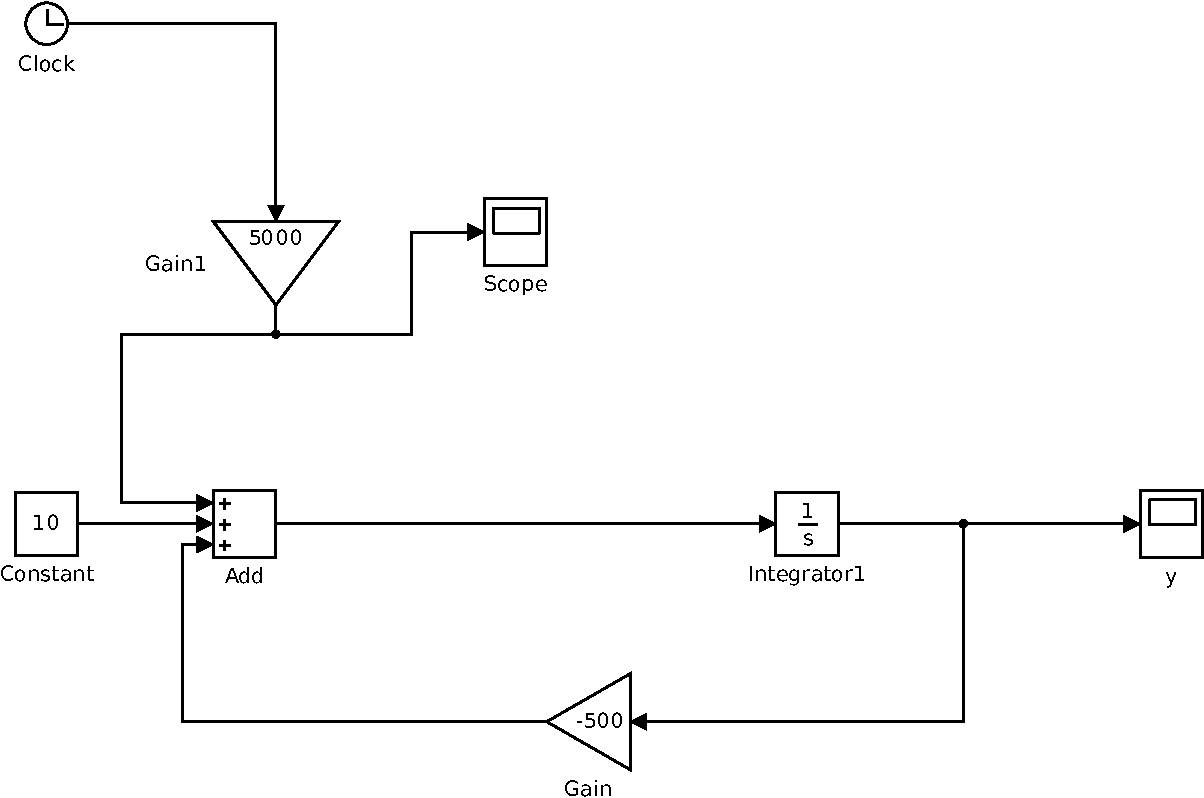
\includegraphics[width=0.9\linewidth]{../screenshots/1}
\end{figure}
\subsection{Geben Sie die Iterationsgleichungen für das Euler-Verfahren an.}
\begin{subequations}
\begin{align}
y_{n+1} = y_n + h * y'(x_n,y_n)\\
x_{n+1} = x_n + h
\end{align}
\end{subequations}

\subsection{Geben Sie die Iterationsgleichungen für das RK2-Verfahren an.}
\begin{subequations}
\begin{align}
k1 = h * y'(x_n,y_n)\\
k2 = h * y'(x_n + \frac{h}{2},y_n + \frac{k1}{2})\\
y_{n+1} = y_n + k2\\
x_{n+1} = x_n + h
\end{align}
\end{subequations}

\subsection{Geben Sie die Iterationsgleichungen für das implizite Euler-Verfahren an.}
\begin{subequations}
\begin{align}
y_{n+1} = y_n + h * (10 - 500 * y_{n+1} + 5000 * x_{n+1})\\
y_{n+1} = y_n + 10 * h - 500 * y_{n+1} * h + 5000 * x_{n+1} * h)\\
y_{n+1} + 500 * y_{n+1} * h = y_n + 10 * h + 5000 * x_{n+1} * h)\\
y_{n+1} * (1+ 500 * h) = y_n + 10 * h + 5000 * x_{n+1} * h)\\
y_{n+1} = \frac{(y_n + 10 * h + 5000 * h * x_n+1)}{ (1+500*h)}
\end{align}
\end{subequations}

\subsection{Schreiben Sie ein Programm "`Stiff.ch"', welches die DGL mit allen Verfahren
löst und zusammen mit der analytischen Lösung in einem Plot anzeigt.}

Siehe Stiff.ch.

\begin{center}
\begin{large}
Versuchsdurchführung
\end{large}
\end{center}


\section{Lösung einer (nichtlinearen) DGL 2. Ordnung (Van-der-Pol-DGL) mit RK 2}
\subsection{Geben Sie das Analogrechner-/Simulink-Schaltbild an.}
\begin{figure}[h]
\centering
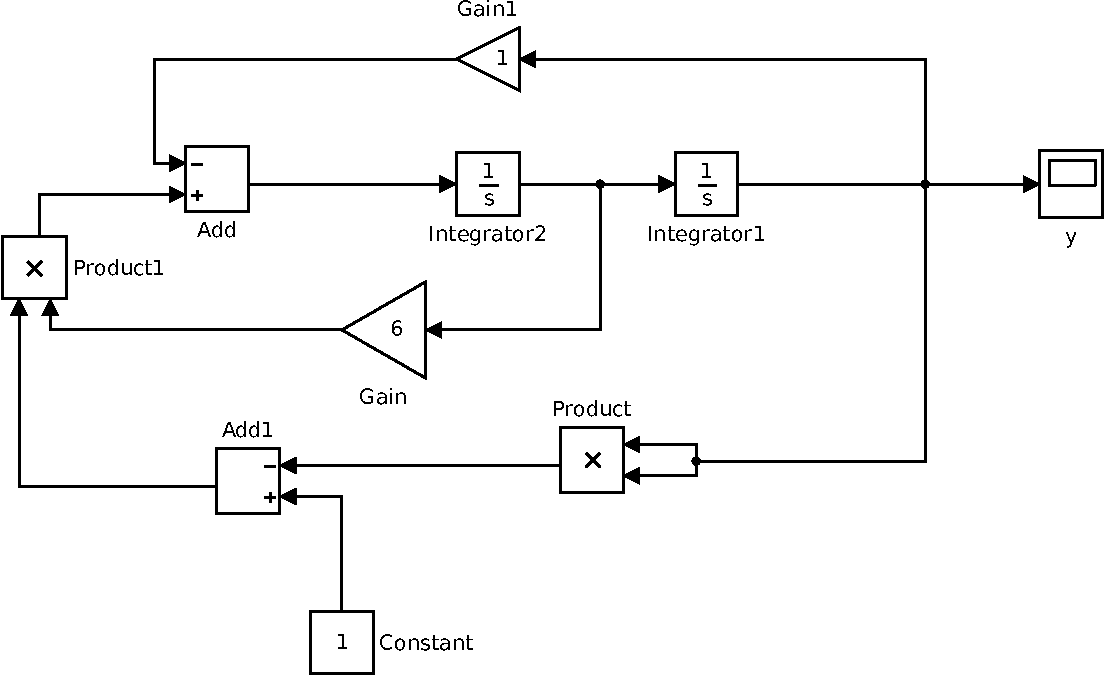
\includegraphics[width=0.9\linewidth]{../screenshots/2}
\end{figure}

\subsection{Geben Sie die DGL 2. Ordnung als 2 DGLn 1. Ordnung an.}

\subsection{Geben Sie die Iterationsgleichungen für das Euler-Verfahren an.}

\subsection{Geben Sie die Iterationsgleichungen für das RK2-Verfahren an.}

\subsection{Schreiben Sie ein Programm "VanDerPol.ch", welches die DGL mit beiden
Verfahren löst und in einem Plot anzeigt.}

\begin{center}
\begin{large}
Versuchsdurchführung
\end{large}
\end{center}

\section{Lösung eines Differentialgleichungssystems (Lorenz-Attraktor) mit RK 2}
\subsection{Geben Sie die Iterationsgleichungen für das RK2-Verfahren an.}
\begin{subequations}
\begin{align}
k_{1x} = -10 * h * (x_n - y_n)\\
k_{1y} = h * [(40-z_n) * x_n - y_n]\\
k_{1z} = h * [(x_n * y_n) - (2,67 * z_n)]\\
k_{2x} = -10 * h * [(x_n +\frac{k_{1x}}{2}) - (y_n + \frac{k_{1y}}{2})]\\
k_{2y} = h * [(40 - z + \frac{k_{1z}}{2}) * (x + \frac{k_{1x}}{2}) - (y_n + \frac{k_{1y}}{2})]\\
k_{2z} = h * [(x + \frac{k_{1x}}{2}) * (y + \frac{k_{1_y}}{2}) - 2,67 * (z + \frac{k_{1z}}{2})]
\end{align}
\end{subequations}

\subsection{Schreiben Sie ein Programm "Lorenz.ch", welches das DGL-System löst.
Geben Sie im 1. Plot die Funktion x(t) aus:
Geben Sie im 2. Plot z(x) aus.}

\subsection{Realisieren Sie das Differentialgleichungssystem mit MATLab/Simulink}
\begin{figure}[h]
\centering
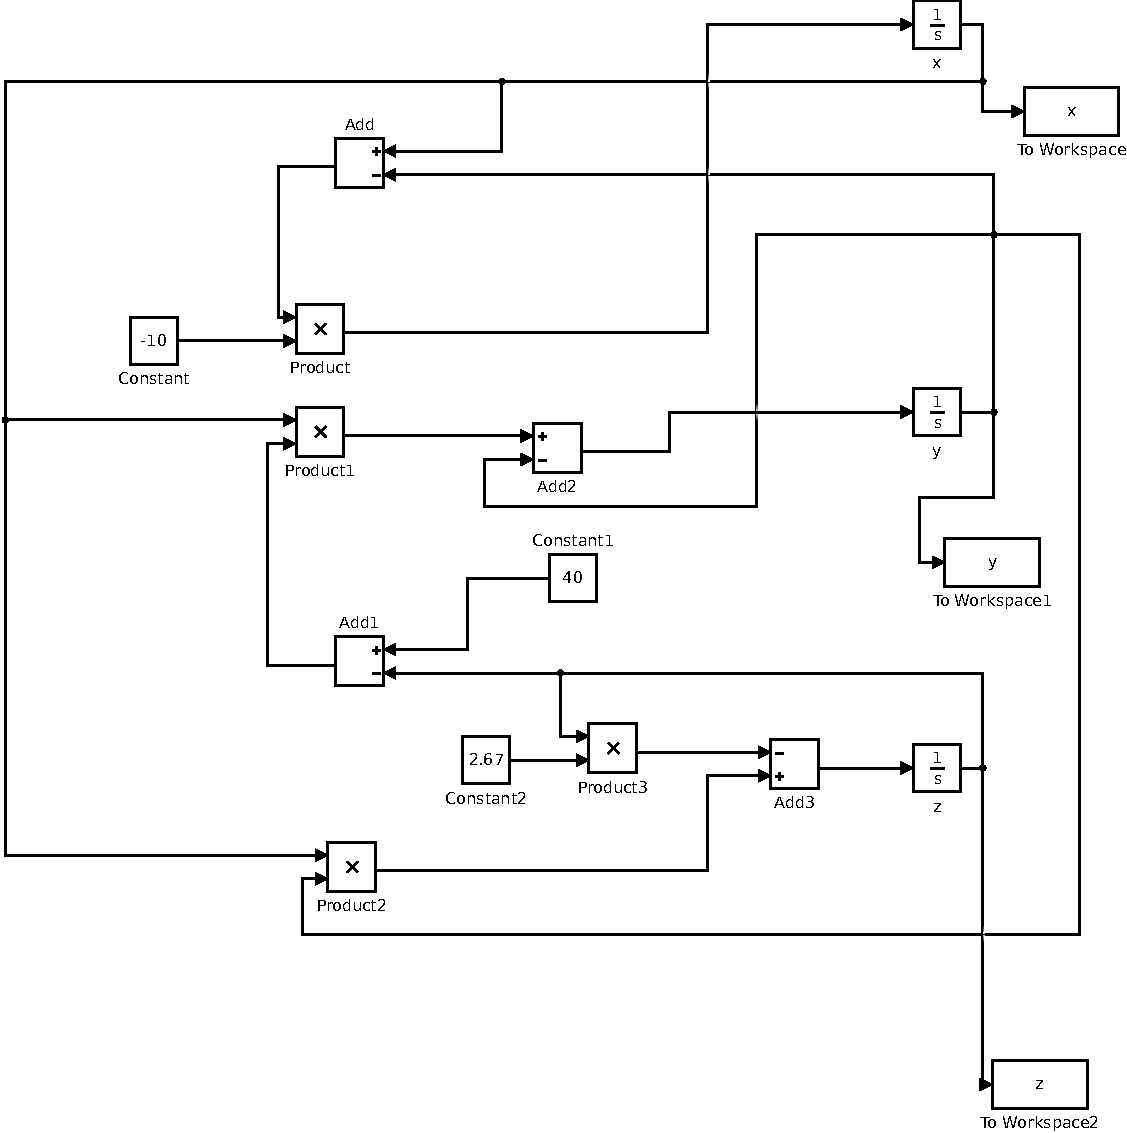
\includegraphics[width=0.9\linewidth]{../screenshots/3}
\end{figure}

\begin{center}
\begin{large}
Versuchsdurchführung
\end{large}
\end{center}

\end{document}